\documentclass[12pt]{beamer}
\setbeamertemplate{navigation symbols}{}%remove navigation symbols
\usepackage{booktabs}
\usepackage{multicol}
\usepackage{transparent}
\usepackage{soul}
\usepackage{wasysym}
\usepackage{hyperref}
\usepackage{subcaption}
\usepackage{listings}
\usepackage{fancyvrb}
\usepackage{multicol}
\usepackage{booktabs}
\usepackage[document]{ragged2e}
\usepackage[english]{babel}
\usepackage{blindtext}
\usepackage{ragged2e}
\usepackage{adjustbox}
\usepackage{amsmath}
\usepackage{tcolorbox}
\usepackage{graphicx}
\usepackage{animate}
\captionsetup{justification=raggedright,singlelinecheck=false}

\newenvironment{myenv}[1]
  {\mdfsetup{
    frametitle={\colorbox{white}{\space#1\space}},
    innertopmargin=0pt,
    frametitleaboveskip=-\ht\strutbox,
    frametitlealignment=\center,
    linewidth=1pt,
    roundcorner=10pt
    }
  \begin{mdframed}%
  }
  {\end{mdframed}}

\useoutertheme{infolines}
\usepackage{newpxtext,newpxmath}
%\usepackage{mathpazo}

\usepackage[framemethod=tikz]{mdframed}
\usetikzlibrary{shadows}
\usepackage{pdfpages}
\newmdenv[shadow=true,shadowcolor=black,font=\sffamily,rightmargin=8pt]{shadedbox}
\usepackage{pifont,xcolor}
\definecolor{myblue}{RGB}{49,54,149}
\definecolor{myred}{RGB}{165,0,38}

\definecolor{myorange}{RGB}{255,120,0}
\definecolor{mygreen}{RGB}{76, 187, 23}

\definecolor{grayedout}{RGB}{225,225,225}
\usepackage{graphicx}
\usepackage{caption}
\usepackage{amsmath}
\newcommand{\icol}[1]{% inline column vector
  \left(\begin{smallmatrix}#1\end{smallmatrix}\right)%
}
\newcommand{\lenitem}[2][.55\linewidth]{figures//\parbox[t]{#1}{#2\strut \strut \justify \justifying}}

\usetheme{Frankfurt}

%   \usefonttheme{professionalfonts}
\newenvironment{variableblock}[3]{%
  \setbeamercolor{block body}{#2}
  \setbeamercolor{block title}{#3}
  \begin{block}{#1}}{\end{block}}
\usecolortheme{dove}
%\usecolortheme{rose}
%\usecolortheme{whale}

\usefonttheme[onlymath]{serif}  % only math serif font
\usefonttheme{serif}

\setbeamercolor{block title}{bg=white,fg=black}
\newcommand{\itemcolor}[1]{% Update list item colour
  \renewcommand{\makelabel}[1]{\color{#1}\hfil ##1}}

\newcounter{tmpc}
\setbeamercolor{section in head/foot}{fg=black, bg=white}
\setbeamercolor{enumerate item}{ fg=myred}
\setbeamertemplate{frametitle}
{
    \nointerlineskip
    \begin{beamercolorbox}[sep=0.3cm,ht=1.8em,wd=\paperwidth]{frametitle}
        \vbox{}\vskip-3ex%
        \strut\insertframetitle\strut
        \vskip-1.2ex%
    \end{beamercolorbox}
}
\addtobeamertemplate{frametitle}{\vskip0.5ex}{}
\makeatletter
\setbeamertemplate{footline}
{
  \leavevmode%
  \hbox{%
  \begin{beamercolorbox}[wd=.875 \paperwidth,ht=2.25ex,dp=1ex,left]{section in head/foot}%
    \usebeamerfont{author in head/foot}\quad \quad \insertshorttitle
 \end{beamercolorbox}%
 \begin{beamercolorbox}[wd=.125\paperwidth,ht=2.25ex,dp=1ex,right]{section in head/foot}%
    \usebeamerfont{date in head/foot} \quad \quad
    \insertframenumber{} / \inserttotalframenumber\hspace*{2ex}
  \end{beamercolorbox}}%
  \vskip0pt%
}
\let\@@magyar@captionfix\relax



\newcommand\jsonkey{\color{purple}}
\newcommand\jsonvalue{\color{cyan}}
\newcommand\jsonnumber{\color{orange}}

% switch used as state variable
\makeatletter
\newif\ifisvalue@json

\lstdefinelanguage{json}{
    tabsize             = 4,
    showstringspaces    = false,
    keywords            = {false,true},
    alsoletter          = 0123456789.,
    morestring          = [s]{"}{"},
    stringstyle         = \jsonkey\ifisvalue@json\jsonvalue\fi,
    MoreSelectCharTable = \lst@DefSaveDef{`:}\colon@json{\enterMode@json},
    MoreSelectCharTable = \lst@DefSaveDef{`,}\comma@json{\exitMode@json{\comma@json}},
    MoreSelectCharTable = \lst@DefSaveDef{`\{}\bracket@json{\exitMode@json{\bracket@json}},
    basicstyle          = \ttfamily
}

% enter "value" mode after encountering a colon
\newcommand\enterMode@json{%
    \colon@json%
    \ifnum\lst@mode=\lst@Pmode%
        \global\isvalue@jsontrue%
    \fi
}

% leave "value" mode: either we hit a comma, or the value is a nested object
\newcommand\exitMode@json[1]{#1\global\isvalue@jsonfalse}

\lst@AddToHook{Output}{%
    \ifisvalue@json%
        \ifnum\lst@mode=\lst@Pmode%
            \def\lst@thestyle{\jsonnumber}%
        \fi
    \fi
    %override by keyword style if a keyword is detected!
    \lsthk@DetectKeywords%
}


\makeatother

\def\mf{
\begin{itemize}
\item Item
\end{itemize}
}
\setbeamercolor{item projected}{bg=myblue}
\setbeamertemplate{enumerate items}[default]
\setbeamertemplate{navigation symbols}{}
%\setbeamercovered{transparent}
\setbeamercolor{block title}{fg=myred}
\setbeamercolor{local structure}{fg=myred}

\usepackage{listings}

\lstdefinestyle{BashInputStyle}{
  language=bash,
  basicstyle=\small\sffamily,
  numbers=left,
  numberstyle=\tiny,
  numbersep=5pt,
  framexleftmargin=3mm,
  frame=shadowbox, rulesepcolor=\color{gray},
  numberstyle=\normalfont\tiny\color{myred},
  rulecolor=\color{black},
  columns=fullflexible,
  backgroundcolor=\color{white},
  linewidth=0.9\linewidth,
  xleftmargin=0.1\linewidth
}

\begin{document}

\section{Introduction and Motivation}
\setstcolor{red}

\title{On the Responsible use of Pseudo-Random Number Generators in Scientific Research} \vspace{-0.25in}
\author{\footnotesize{Charlie Rahal\\ \vspace{0.05in} LCDS and Nuffield College, University of Oxford\\\vspace{.1in}Ox | Ber 2023}\\ \vspace{-0.15in}}
 \date{}
\frame{\titlepage
\begin{center}
\vspace{-.6in}
\begin{figure}
\centering
\begin{subfigure}{.5\textwidth}
  \centering
  \includegraphics[width=.55\linewidth]{figures/LCDS_Logo_SVG_BlackOrange.pdf}
\end{subfigure}%\hspace{-.05in}
\hspace{.01in}\begin{subfigure}{.45\textwidth}
  \centering
  \includegraphics[width=.45\linewidth]{figures//Uni_Oxford_logo.pdf}
\end{subfigure}
\end{figure}
 \end{center}
}

\begin{frame}
\frametitle{Pseudo-Random Number Generation}
An invisible source of uncertainty in the scientific record: PRNGs! \\ \vspace{.05in} \pause
	\begin{itemize}
		\item \textbf{Q}: Has anyone ran a program twice, with different results?\\ \vspace{.1in}\pause
		\item \textbf{Q}: Has anyone here ever set a `\color{myblue}seed\color{black}'? Which seed?\\ \vspace{.1in}\pause
		\item Maybe to eliminate variation in algorithms with PRNGs?\\ \vspace{.05in}
		\begin{itemize}
		\item[-] This seems to be the current `best practice' advice.\\ \vspace{.1in}  \pause
		\end{itemize}
			\item We argue this is the \color{myred}opposite of what we want\color{black}!\\ \vspace{.05in}
			\begin{itemize}
				\item[-] We propose you pre-specify \textbf{multiple} (complex) seeds.
			\end{itemize}
	\end{itemize}
\end{frame}

\begin{frame}
\frametitle{Pseudo-Random Number Generation (Cont.)}
	\begin{itemize}
 		\item We want to consider possible variation independent of arbitrary variation in seed choice.\vspace{.1in}\pause
		\item This is an extremely important and scarcely research problem.\vspace{.1in}\pause
		\item Pseudo-Random Number Generators occur \color{myblue}everywhere\color{black}!\\ \vspace{.1in}\pause
		\item The variation in estimand can be \color{myblue} \textbf{huge}\color{black}.\\ \vspace{.1in}\pause
		\item We bring attention to this through multiple types of replications.\\ \vspace{.05in}
		\begin{itemize}
			\item Simulations, machine learning, and inferential research.
		\end{itemize}
	\end{itemize}
\end{frame}


\begin{frame}
\begin{itemize}
\item \textbf{\color{myred}Problem Statement\color{black}}: By setting one seed, we have no idea about the potential key variation of our estimand as a function of how random numbers were generated. This is computationally un-intensive, but scientifically dour.\\ \pause \vspace{.2in}
\item \textbf{\color{myred}Solution\color{black}}: Visualize the outcome space of a of large number (10k? 100k?) seeds simultaneously. This is computationally intensive, but scientifically faithful.\\ \pause \vspace{.2in}
\item \textbf{\color{myred}Replication\color{black}}: We can consider whether an original result is in the tail of our distribution (or IQR?) or not.\\ \vspace{.2in}
\end{itemize}
\end{frame}


\section{Simple Simulations}
\begin{frame}
\begin{center}
\begin{figure}
	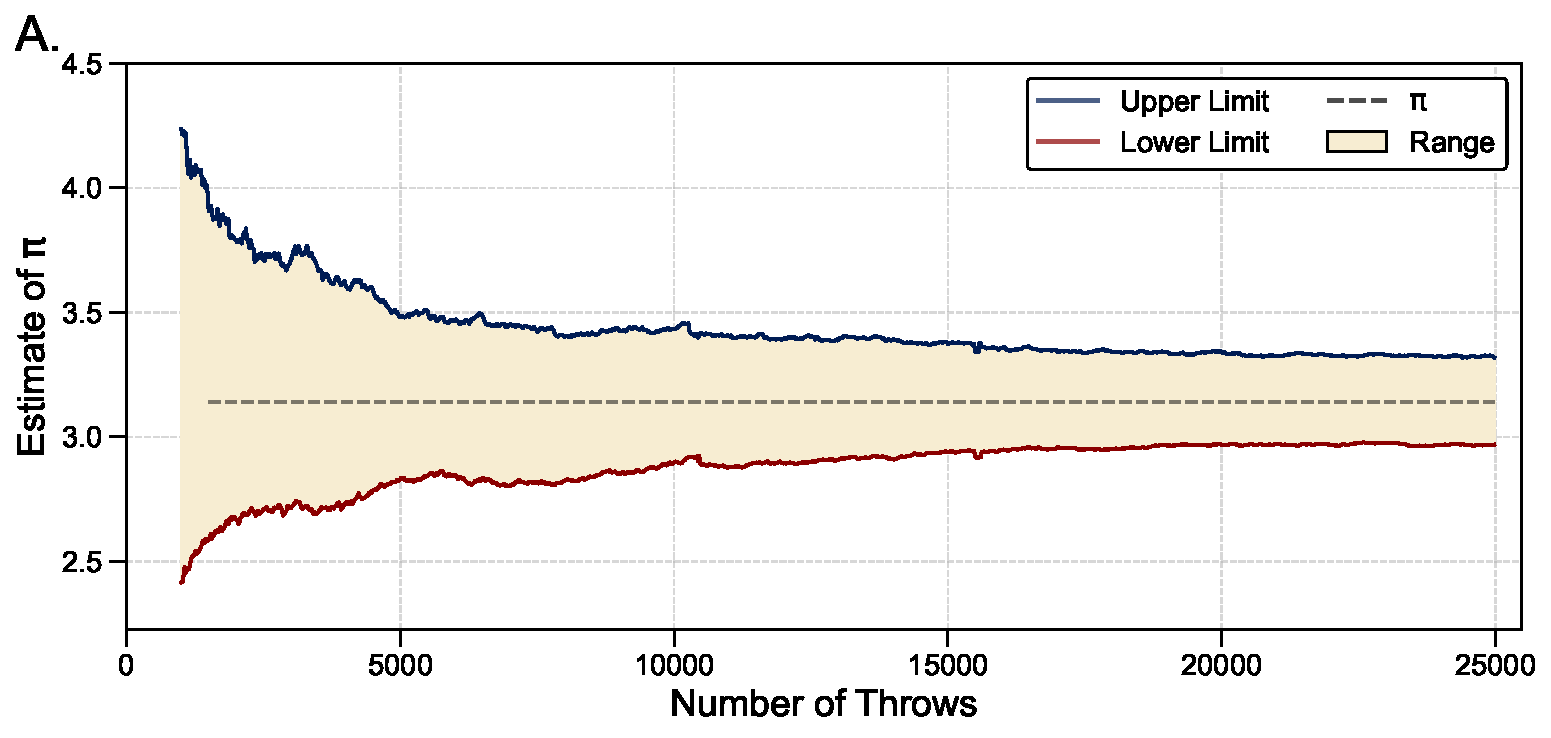
\includegraphics[width=\textwidth]{../../figures//buffon_seeds.pdf}
\end{figure}
\end{center}
\end{frame}

\section{Machine Learning}
\begin{frame}
\begin{center}
\begin{figure}
	\includegraphics[width=\textwidth]{../../figures//prediction_seeds_a.pdf}
\end{figure}
\end{center}
\end{frame}

\section{Other Examples}
\begin{frame}
\begin{center}
\begin{figure}
	\includegraphics[width=0.95\textwidth]{../../figures//two_various.pdf}
\end{figure}
\end{center}
\end{frame}

\section{Replication}
\begin{frame}
\begin{center}
\begin{figure}
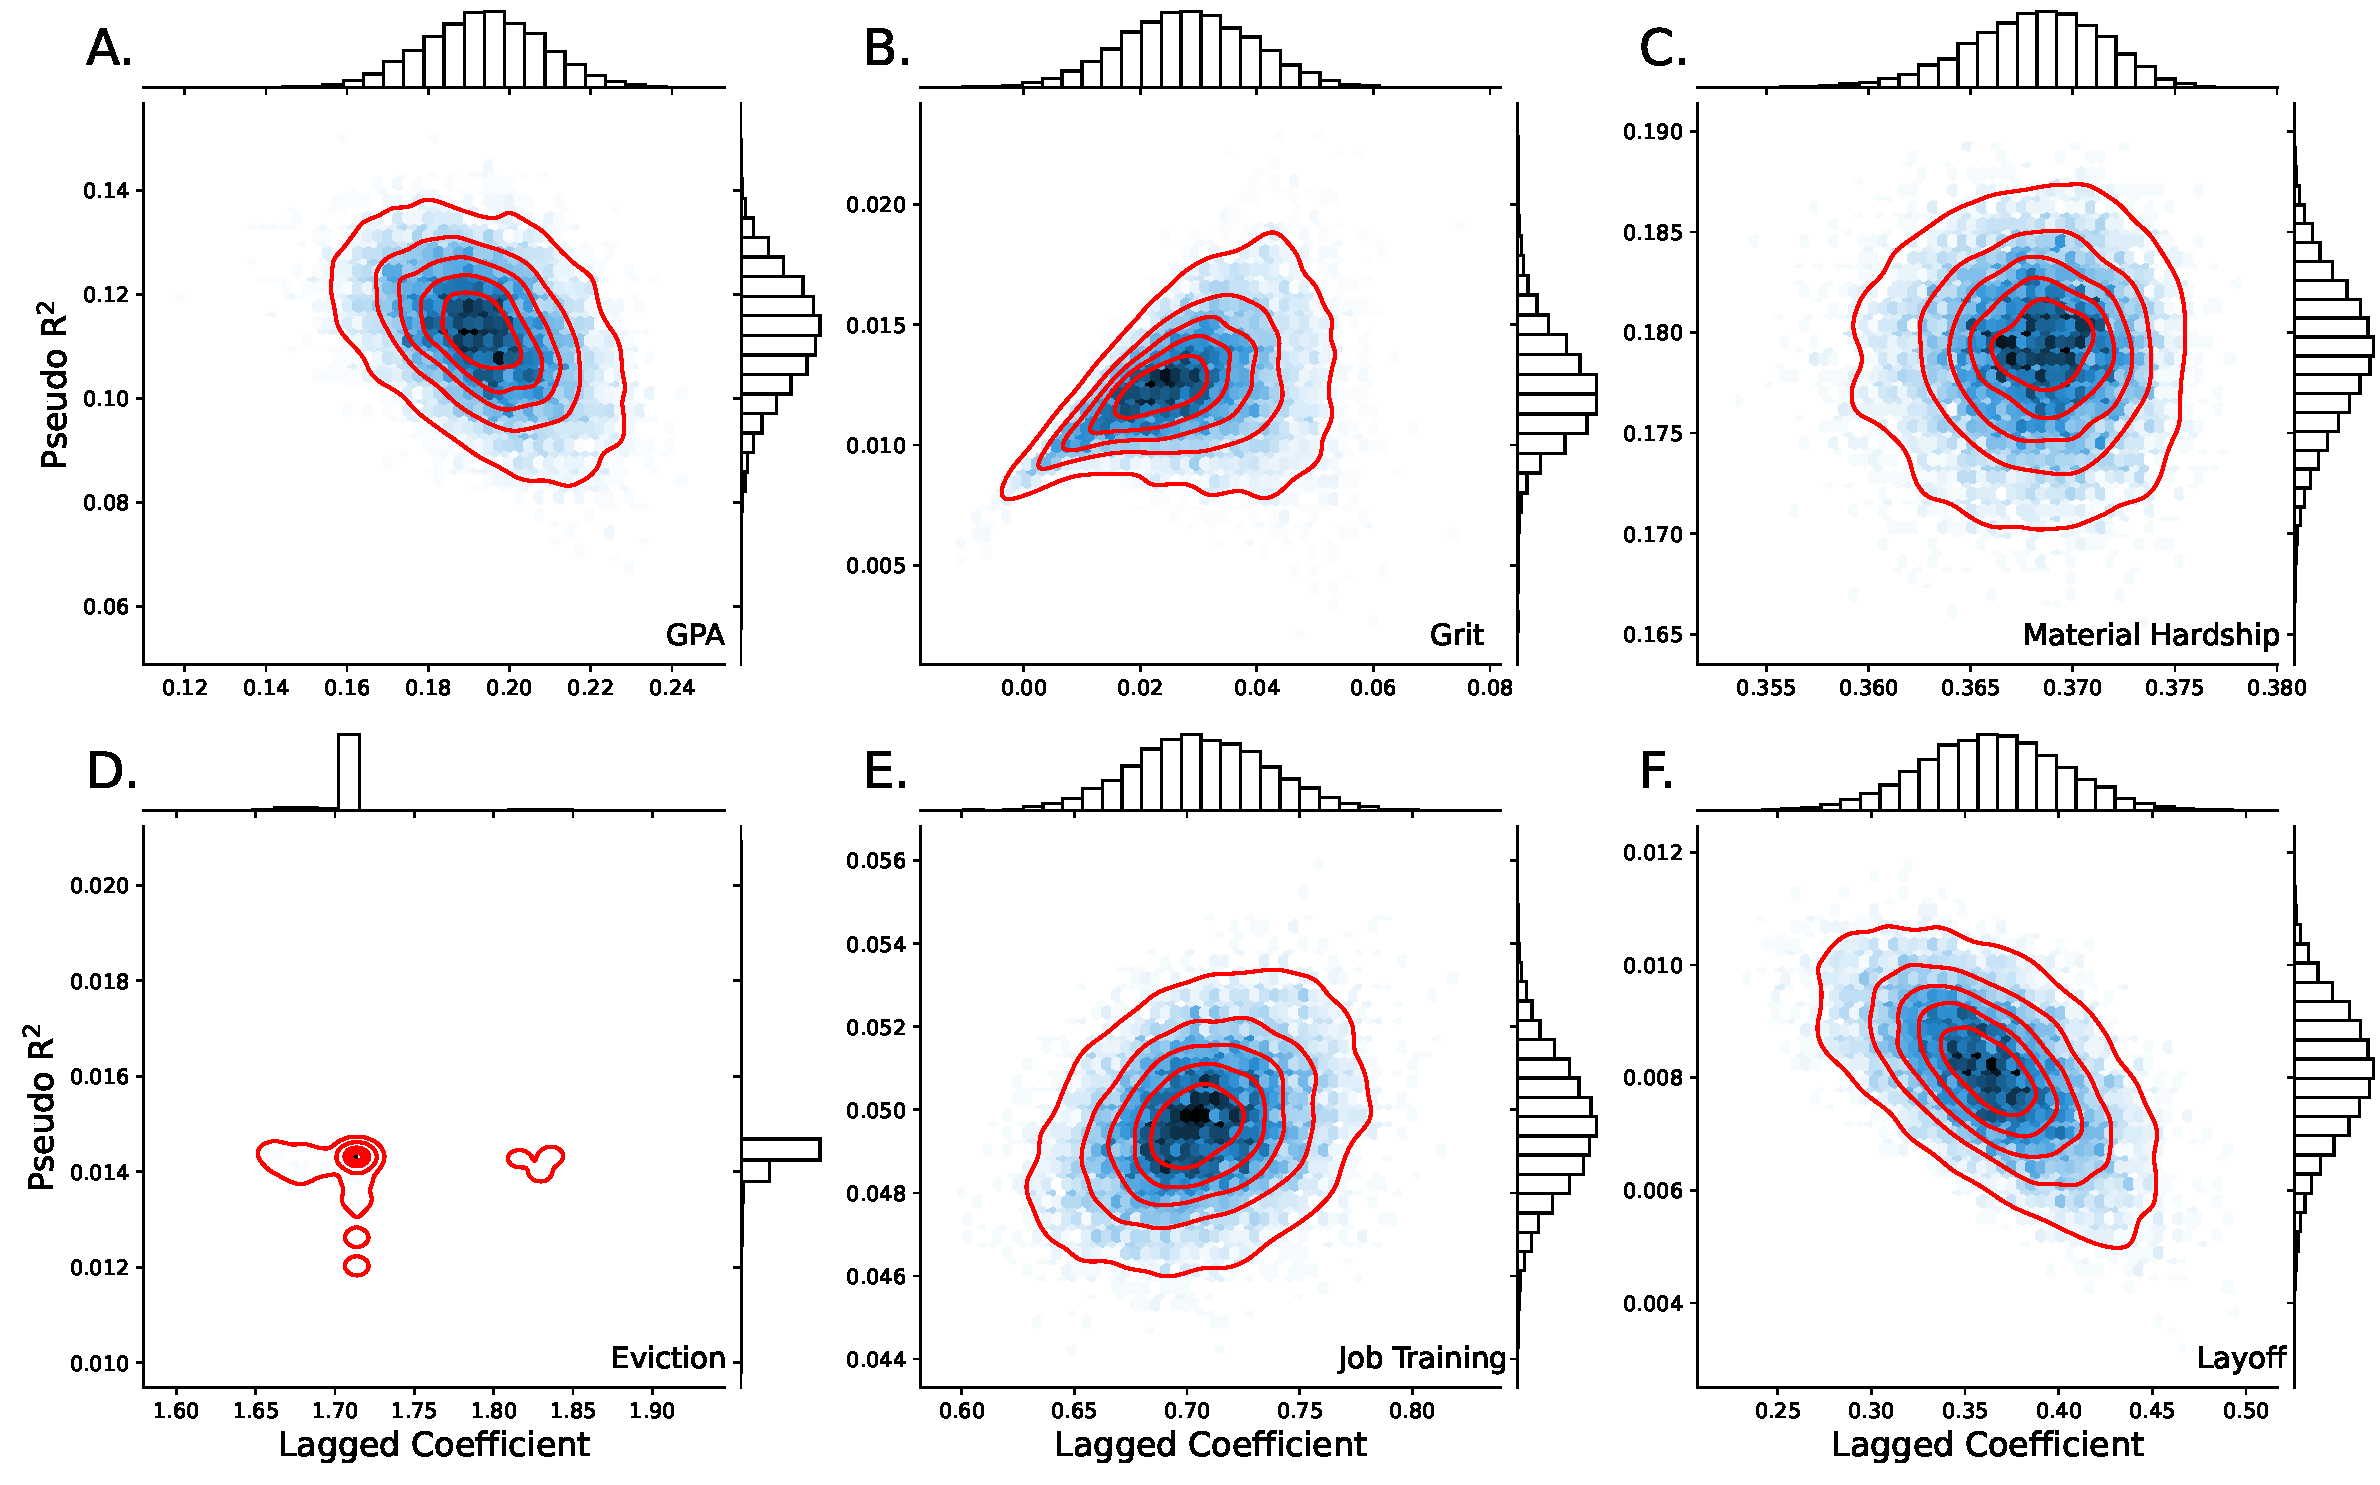
\includegraphics[width=.925\linewidth]{../../figures//ffc_seeds.pdf} \\ \vspace{.025in}
\end{figure}
\end{center}
\end{frame}

\section{Next Steps}
\begin{frame}
\frametitle{\color{myred}What's Next?{} \color{black} Indexing Seed Variability}
\begin{itemize}
\item The next thing to do is to formalize the replication project.\\ \vspace{.1in}
\begin{itemize}
\item[-] Does anyone have ideas for other types of seed variability?\\ \vspace{.1in}
\end{itemize}
\item We are seeking to make a project website, which:\\ \vspace{.1in}
\begin{enumerate}
\item Provides (a set of) seeds (already downloadable on GitHub).\\ \vspace{.1in}
\item Indexes examples of seed variability in existent papers.\\ \vspace{.1in}
\end{enumerate}
\item The first improves the future of the scientific record.\\ \vspace{.1in}
\item The second makes the historic scientific record more robust.\\ \vspace{.1in}
\end{itemize}
\end{frame}

\end{document}
